\subsection{UC2 - Registrazione come amministratore}\label{usecase:2}

\begin{figure}[H]
    \centering
    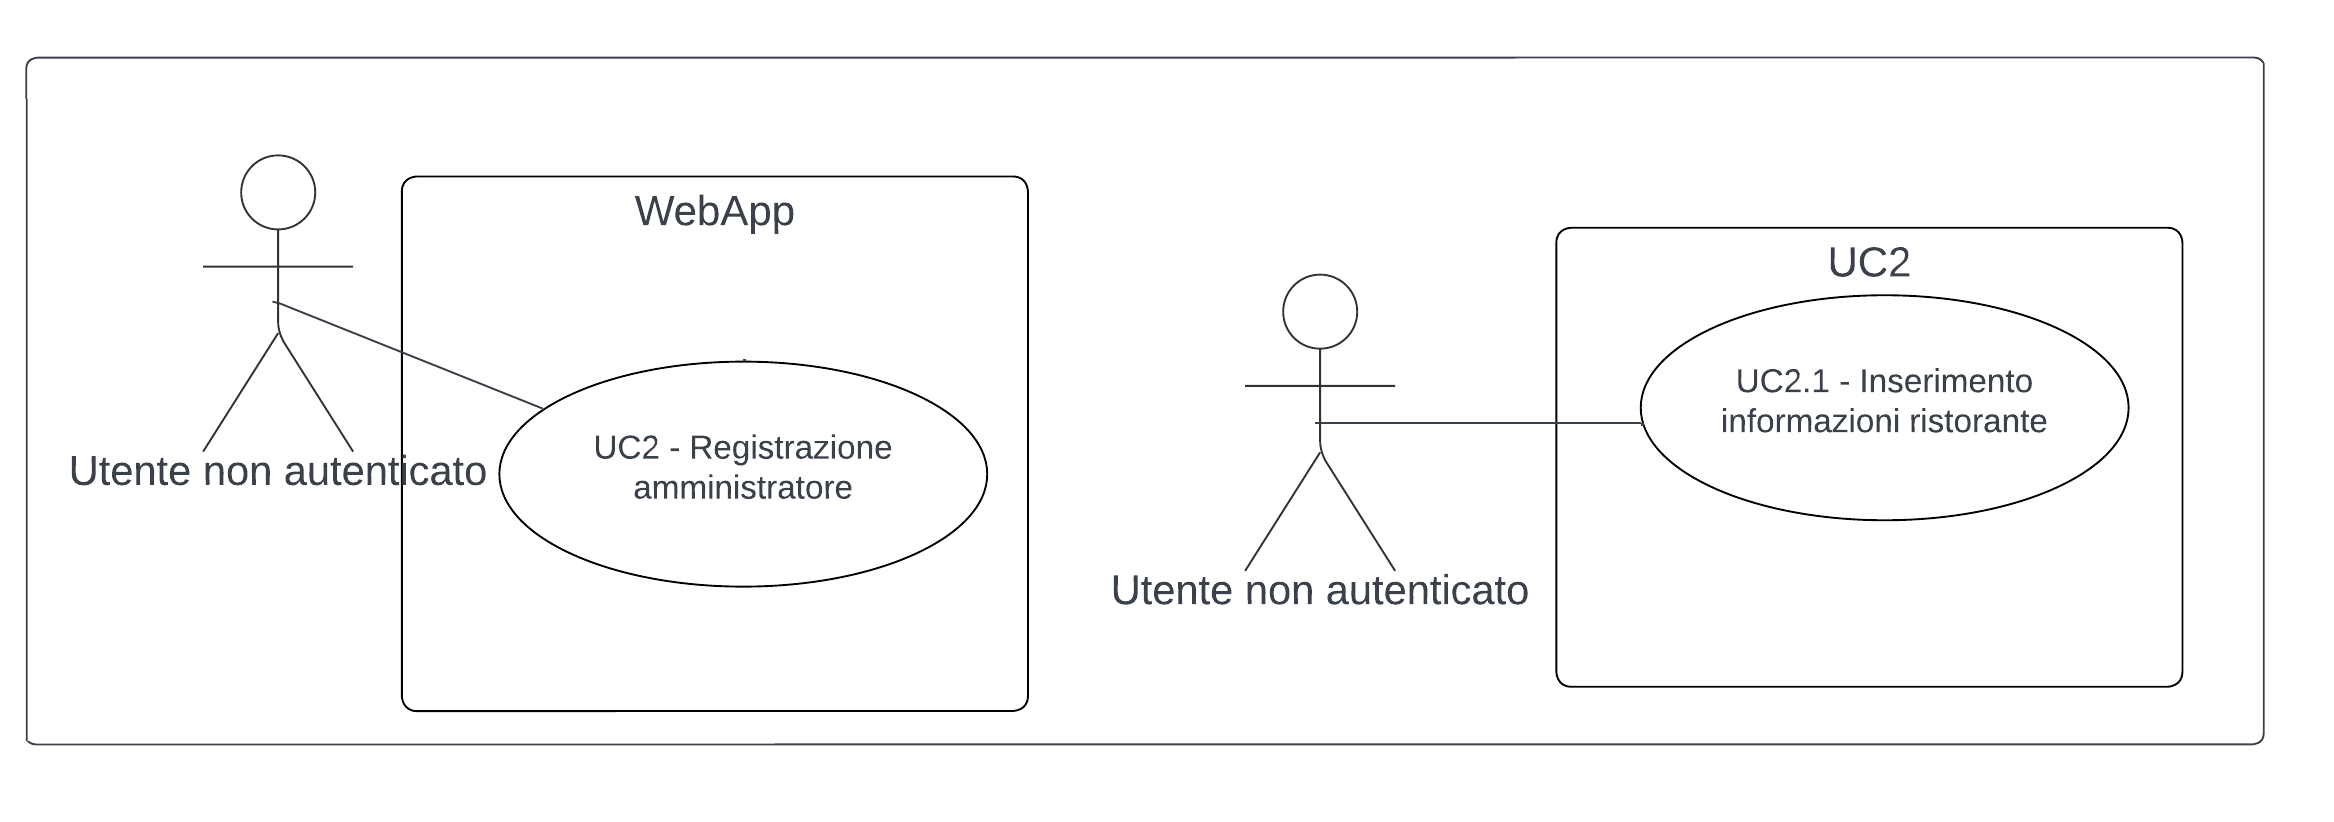
\includegraphics[width=0.9\linewidth]{ucd/UCD2_corretto.png}
\caption{Registrazione come amministratore}
\end{figure}

\textbf{Attori principali}: 
\begin{itemize}
    \item Utente non autenticato.
\end{itemize}
\textbf{Precondizioni}:
\begin{itemize}
    \item L'utente è connesso al $\textit{Sistema}_G$;
    \item L'utente ha ricevuto un link di invito speciale che permette la registrazione come amministratore.
\end{itemize}
\textbf{Postcondizioni}: 
\begin{itemize}
    \item L'utente si è registrato ed è riconosciuto dal $\textit{Sistema}_G$ come amministratore.
\end{itemize}
\textbf{Scenario principale}:
\begin{enumerate}
    \item L'utente inserisce il nome;
    \item L'utente inserisce il cognome;
    \item L'utente inserisce un'email valida;
    \item L'utente inserisce la password che rispetta i criteri indicati;
    \item L'utente inserisce le informazioni del ristorante (\nameref{usecase:2_1}).
\end{enumerate}
\textbf{Scenari alternativi}:
\begin{itemize}
    \item 1.1.  L'utente lascia il campo nome vuoto;
    
    1.2.  L'utente lascia il campo cognome vuoto;
    
    1.3a.  L'utente lascia il campo email vuoto;
    
    1.3b.  L'utente non inserisce una email nel formato: xxxxx@yyy.zz;
    
    1.3c.  L'utente inserisce una email già registrata;
    
    1.4a.  L'utente lascia il campo password vuoto;
    
    1.4b.  L'utente inserisce una password troppo corta (minore di 6 caratteri);
    
    1.4c.  L'utente inserisce una password troppo lunga (maggiore di 24 caratteri);
    
    1.4d.  L'utente inserisce una password senza caratteri minuscoli;
    
    1.4e.  L'utente inserisce una password senza caratteri maiuscoli;
    
    1.4f.  L'utente inserisce una password senza caratteri numerici;
    
    1.4g.  L'utente inserisce una password senza caratteri speciali;

    1.5.  L'utente lascia il campo nome ristorante vuoto;

    1.6.  L'utente lascia il campo città vuoto;
    
    1.7.  L'utente lascia il campo recapiti del ristorante vuoto;
    
    1.8.  L'utente lascia il campo orario apertura vuoto;
    
    1.9.  L'utente lascia il campo coperti disponibili vuoto;
    
    1.10.  L'utente lascia il campo tipologia cucina vuoto;
    
    2.  Viene visualizzato un errore esplicativo;
    
    3.  Viene data la possibilità di rifare la registrazione come amministratore;
    \item L'utente decide di annullare l'operazione di registrazione.
\end{itemize}